\section{Introduction}
\label{sec:intro}

Text-to-Image (T2I) diffusion models~\cite{rombach2022highresolution,pernias2023stablecascade} have revolutionized digital content creation, demonstrating remarkable capabilities in synthesizing highly detailed and visually stunning images from natural language descriptions. However, verbalizing complex artistic styles---encompassing nuanced brushstrokes, non-Euclidean textures, delicate color harmonies, and specialized medium properties (e.g., stained glass, woodblock printing, origami, neon cyberpunk)---remains exceptionally difficult through text prompts alone. Consequently, visual style personalization via reference image exemplars has emerged as a crucial paradigm in computer vision and generative AI.

Despite notable advancements, existing style transfer and personalization techniques grapple with two persistent, interrelated bottlenecks:

% ==============================================================================
% Teaser Figure: Comprehensive Qualitative Matrix (Content x Style)
% Exported directly from the interactive OrthoStyle Visualizer Web App
% ==============================================================================
\begin{figure*}[t]
\centering
\includegraphics[width=\textwidth]{figs/qualitative_matrix_teaser.png}
\caption{\textbf{Qualitative Stylization Matrix of \method across Diverse Content Categories and Artistic Styles.} 
Rows depict representative content exemplars spanning multiple semantic domains (animals, vehicles, everyday objects, and architecture); columns correspond to challenging artistic styles (classical oil paintings, stained glass, mosaic tile art, Japanese woodblock prints, glowing neon cyberpunk, and 3D renders). 
\method demonstrates faithful subject identity, pose, and silhouette retention while authentically rendering complex artistic brushwork and material textures without semantic leakage.}
\label{fig:teaser_matrix}
\end{figure*}

\paragraph{Bottleneck 1: Severe Content Leakage.} 
Artistic reference images are rarely pure abstract textures; they typically depict concrete semantic objects (e.g., a reference painting featuring a starry sky over a village, or a golden sculpture of a dragon). Existing training-free methods~\cite{hertz2023stylealigned,wang2024instantstyle,ye2023ipadapter} frequently extract entangled visual representations via global CLIP or cross-attention embeddings. When injected naively into the generative process through linear feature summation or standard attention manipulation, semantic tokens from the style image inadvertently bleed into the generated image (e.g., generating extraneous dragons or houses when only the golden melting material was desired).

\paragraph{Bottleneck 2: Content Preservation vs. Style Fidelity Dilemma.}
A perennial challenge in neural style transfer is the delicate balance between structural preservation of the target subject and radical stylistic transformation. Aggressive style injection frequently collapses the geometric outlines, facial contours, and spatial poses of the target object, reducing it to an unrecognizable abstract pattern. Conversely, over-constraining the content via rigid spatial adapters or unconditional edge maps often produces lifeless color tinting that completely misses the rich texture, artistic stroke dynamics, and medium alterations of the reference style.

\paragraph{Limitations of Prior Approaches.}
Recent methods such as RB-Modulation~\cite{rout2024rbmodulation} formulate reference-based modulation via stochastic optimal control. While innovative, prior works exhibit critical shortcomings:
\begin{itemize}
    \item \textbf{Naive Linear Feature Combination}: Blending attention tokens via linear addition $\bx = \sum w_k \bx_k$ causes constructive and destructive feature interference, directly inducing content leakage.
    \item \textbf{Off-Manifold Latent Distortion}: Adding unconstrained external guidance gradients into the diffusion sampling loop forces latent trajectories off the legitimate data manifold, leading to oversaturated artifacts and blurry outputs.
    \item \textbf{Fragile DDIM Inversion}: Relying on deterministic inversion of the content image leads to severe error accumulation and unnatural structural rigidity.
\end{itemize}

\paragraph{Our Proposal: \method.}
To decisively resolve these dilemmas, we present \textbf{\method}, an end-to-end training-free style transfer framework designed on top of modern cascaded diffusion architectures (Stable Cascade~\cite{pernias2023stablecascade}). \method fundamentally re-engineers feature interaction and guidance dynamics through geometric orthogonality and temporal scheduling.

\begin{figure}[t]
\centering
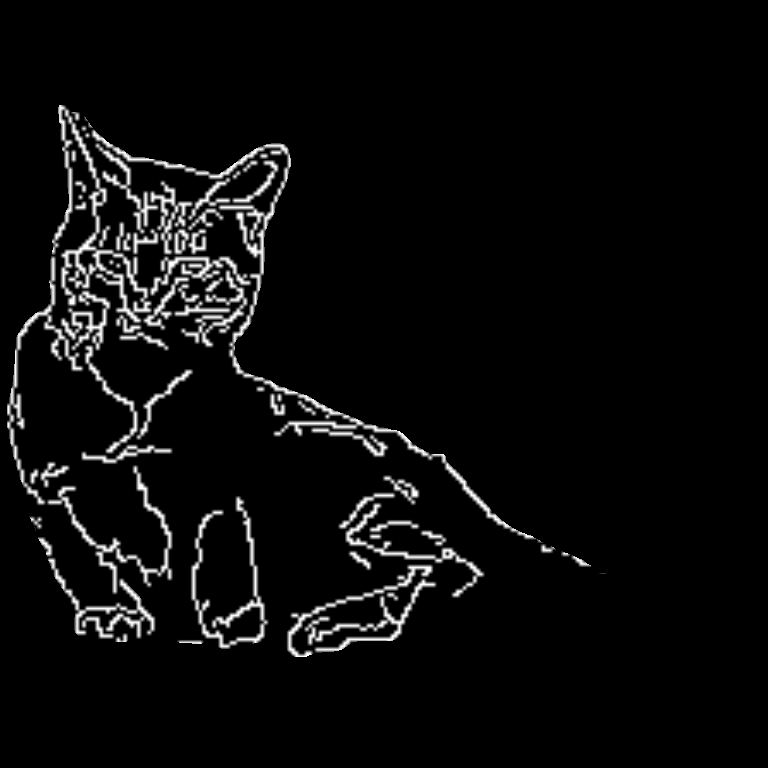
\includegraphics[width=0.95\columnwidth]{figs/canny_edge_map.png}
\caption{\textbf{Semantic Gated Structural Boundary.} Semantic edge extraction via background removal and hard-thresholded gating, isolating target subject geometry from background noise.}
\label{fig:canny_gating}
\end{figure}

\paragraph{Summary of Contributions.}
Our primary contributions are summarized as follows:
\begin{enumerate}
    \item \textbf{Orthogonal Feature Projection with Energy Compensation (Attention-Level)}: We mathematically formulate the style-content interaction in the cross-attention layer as an orthogonal projection onto the null space of the content feature $\Vortho$. To counteract the inevitable norm attenuation caused by projection, we propose an energy compensation mechanism that preserves the full $L_2$ norm of style representations, eradicating content leakage while maximizing artistic expression.
    \item \textbf{Score-Orthogonal DINO Guidance on Latent Manifold (Sampling-Level)}: We design a terminal guidance loss in the self-supervised DINO-ViT feature space~\cite{caron2021emerging}, which captures multi-scale artistic textures without semantic category entanglement. Crucially, we project the guidance gradient onto the subspace orthogonal to the diffusion score vector $\beps_\theta$, guaranteeing that trajectory updates remain strictly tangent to the score manifold and preventing out-of-distribution drift.
    \item \textbf{Temporal Sigmoid-Scheduled AFA and Clean Latent Pushforward}: We implement an Adaptive Feature Allocation (AFA) mechanism governed by an analytical Sigmoid time schedule. This enforces a smooth phase transition from structural skeleton grounding in early timesteps to high-fidelity style crystallization in later timesteps, complemented by an AdaIN clean-latent ($x_0$) pushforward to instantly establish global color tone.
\end{enumerate}
Through comprehensive theoretical justifications, experimental protocols, metric definitions, and ablation baselines, we show that \method sets a new benchmark in training-free artistic style transfer.
